\chapter{Biblioteka:  RIT}
\label{app:takeMeHome}
\thispagestyle{appendixStyle}

Poniżej opisana biblioteka \textsc{RIT} (ang. \textit{Recoverable Incremental Tree}) stanowi zwieńczenie naszej pracy --- zawiera implementacje wszystkich algorytmów, których pseudokody pojawiły się w~powyższym tekście, zarówno tych klasycznych, imperatywnych, jak i~dotyczących problemów programowania liniowego, bądź całkowitoliczbowego. Całość biblioteki została napisana w~języku \textsc{C++} w~jego najnowszym, dostępnym na chwilę powstawania tego dokumentu, standardzie \textsc{C++14}, z~wykorzystaniem elementów bibliotek stron trzecich, takich jak: \textsc{IBM\textsuperscript{\textregistered} CPLEX\textsuperscript{\textregistered} Optimizer}, \textsc{Graphviz}, \textsc{gTest} oraz \textsc{log4cxx}. Poniższy rozdział zawiera skrócony opis jej funkcjonalności\footnote{Pełen projekt wraz z~jego dokumentacją został umieszczony na zdalnym repozytorium pod adresem: \url{https://github.com/PWrGitHub194238/RIT}.}, sposób instalacji oraz korzystania z~niej w~podstawowym zakresie.

\section{Wymagania i~instalacja}

Całość omawianej biblioteki została zaimplementowana w~środowisku systemu \textsc{Ubuntu 15.10} dla architektury $64$-bitowej, w~związku z~tym wszelkie przykłady oraz wykorzystywane skrypty zostały napisane z~myślą o~użytkownikach systemu z~tej rodziny --- proces kompilacji oraz instalacji biblioteki może się różnić w~zależności od wykorzystywanego systemu operacyjnego. Dodatkowo jeden z~prezentowanych skryptów korzysta z~konsolowego \textsc{API} programu \textsc{Eclipse Mars.1 (4.5.1)}, przystosowanego do pisania w~językach \textsc{C} oraz \textsc{C++} (\textsc{Eclipse CDT}), który posłużył do napisania całości biblioteki, co tym samym czyni go preferowanym narzędziem w~przypadku chęci budowy biblioteki \textsc{RIT} na podstawie jej, udostępnionych na zdalnym repozytorium, źródeł. Poniżej prezentowany proces ma w~tym pomóc. 

\subsection{Struktura projektu}

Prezentowane drzewo katalogów ilustruje strukturę projektu oraz precyzuje położenie wszystkich, istotnych z~punktu widzenia instalacji, skryptów. Nim przejdziemy do budowy biblioteki \textsc{RIT} ze źródeł, zapoznamy się ze wszystkimi ważniejszymi składowymi projektu: \textsc{RIT}, \textsc{RIT\_Library} oraz \textsc{RIT\_Examples}.

\small
\noindent\makebox[\textwidth][c]{%
\begin{minipage}{.3\textwidth}
\dirtree{%
	.1 /.
	.2 \textsf{\textcolor{lgray}{EmptyTeX}}.
	.2 \textsf{\textcolor{lgray}{Presentations}}.
	.2 \textsf{\textcolor{lgray}{References}}.
	.2 \textsf{RIT\_Examples}.
	.3 \textsf{include}.
	.3 \textsf{lib}.
	.3 \textsf{src}.
	.3 \textsf{\textcolor{lgray}{test}}.
	.3 build.bash.
	.3 clean.bash.
	.3 config.bash.
	.3 fullBuild.bash.
	.3 \textcolor{lgray}{Log4cxxConfig.xml}.
	.3 memcheck.bash.
	.3 \textcolor{lgray}{RIT\_Examples.Doxyfile}.
}
\end{minipage}% This must go next to `\end{minipage}`
\begin{minipage}{.3\textwidth}
\dirtree{%
	.1 /.
	.2 \textsf{RIT\_Examples}.
	.3 \textcolor{lgray}{RIT\_Examples\_bac}.
	.3 \textcolor{lgray}{valgrind.supp}.
	.2 \textsf{RIT\_Library}.
	.3 \textsf{src}.
	.3 build.bash.
	.3 clean.bash.
	.3 config.bash.
	.3 fullBuild.bash.
	.3 \textcolor{lgray}{Log4cxxConfig.xml}.
	.3 memcheck.bash.
	.3 \textcolor{lgray}{RIT\_Library.Doxyfile}.
	.3 \textcolor{lgray}{RIT\_Library\_bac}.
	.3 toogleLogs.bash.
	.3 \textcolor{lgray}{valgrind.supp}.
}
\end{minipage}% This must go next to `\end{minipage}`
\begin{minipage}{.3\textwidth}
\dirtree{%
	.1 /.
	.2 \textsf{Scripts}.
	.3 \textsf{\textcolor{lgray}{octave}}.
	.3 \textsf{\textcolor{lgray}{plots}}.
	.3 \textcolor{lgray}{cleanThesis.bash}.
	.3 \textcolor{lgray}{generatePlot.bash}.
	.3 \textcolor{lgray}{randDistance.bash}.
	.3 \textcolor{lgray}{randDistance.pl}.
	.2 \textsf{\textcolor{lgray}{Thesis}}.
	.3 \textsf{\textcolor{lgray}{Documentation}}.
	.3 \textcolor{lgray}{Thesis.pdf}.
	.2 buildProject.bash.
	.2 clean.bash. 
	.2 \textcolor{lgray}{LICENSE}. 
	.2 \textcolor{lgray}{README.md}. 
	.2 RIT\_bac.
}
\end{minipage}}

Zaprezentowana powyżej struktura przedstawia wszystkie główne komponenty projektu, łącznie ze skryptami czy folderami, które nie będą na razie dla nas istotne (zostały one zaznaczone szarym kolorem w~celu lepszej przejrzystości przedstawianej struktury katalogów). Etap budowania oraz uruchamiania aplikacji jest mocno zautomatyzowany, dlatego też, podczas wykonywania wszelkich czynności, będziemy głównie korzystać z~plików, napisanych dla jednej z~najbardziej popularnych powłok systemowych --- skryptów o~rozszerzeniu \textsf{*.bash}. Omówimy teraz przeznaczenie każdego z~nich w~folderach: \textsf{RIT\_Library} oraz  \textsf{RIT\_Examples}, jako że w~znacznym stopniu pokrywają się one ze sobą (są przeznaczone dla dwóch różnych podprojektów, z~czego sposób budowy każdego z~nich jest bardzo podobny).

\dirtree{%
	.1 /.
	.2 \textsf{RIT\_Library} / \textsf{RIT\_Examples}.
	.3 config.bash.
}

Główny skrypt dla projektów \textsc{RIT\_Library} oraz \textsc{RIT\_Examples}. Po wywołaniu wiersza poleceń ( \texttt{CRTL + ALT + T}) i~wykonaniu polecenia \mintinline{bash}|./config.bash| (lub \mintinline{bash}|bash config.bash| w~przypadku, gdy plik skryptu nie posiada atrybutu, określającego go jako plik wykonywalny), ukażą nam się następujące opcje do wyboru:

\begin{minted}[escapeinside=||,mathescape=true,linenos=true,fontsize=\footnotesize]{text}
|# :\textapprox/git/RIT/RIT\_Library\$ ./config.bash|
You have to specify at least one action from these:
	autocompletion
	help
	install
	initBuild
\end{minted}

Wybierając pierwszą z~nich (wpisując w~terminalu \mintinline{bash}|./config.bash autocompletion| i~zatwierdzając swój wybór), zostaniemy poproszeni o~zezwolenie na podwyższenie uprawnień uruchomionego procesu --- w~przypadku wyrażenia zgody, do katalogu systemowego \textsf{\textapprox/etc/bash\_completion.d/} zostanie przeniesiony plik \textsf{RIT\_Library\_bac} (bądź \textsf{RIT\_Examples\_bac}), który umożliwi systemowi operacyjnemu podpowiadanie nam składni wszystkich przyszłych komend (zasugeruje nam także możliwe ich parametry). Aby zmiany wprowadzone przez skrypt były widoczne, wymagane jest ponowne uruchomienie wiersza poleceń (\texttt{CRTL + ALT + T}). Od tej chwili możemy, poprzez podwójne naciśnięcie klawisza \texttt{TAB}, wypisać wszystkie, możliwe do zastosowania w~danej chwili (na podstawie do tej pory wpisanego ciągu znaków w~wierszu poleceń), parametry. Dodatkowo, jeżeli argument określonego parametru powinien spełniać określone właściwości (np. być plikiem wykonywalnym), po naciśnięciu klawisza \texttt{TAB} automatycznie zostanie podpowiedziana jego wartość (jeśli jest tylko jedna możliwa):

\begin{minted}[escapeinside=||,mathescape=true,linenos=true,fontsize=\footnotesize,]{text}
|# :\textapprox/git/RIT/RIT\_Library\$ ./config.bash autocompletion|
In order to successfully execute this commamd, extra privileges will be needed:
	[sudo] [...]
You have granted this script root privileges.
Please, restart shell in order to changes take effect.
\end{minted}

Oczywiście uruchomienie skryptu z, następnym w~kolejności, parametrem \mintinline{text}|help|, spowoduje wypisanie opisu wszystkich, możliwych do zastosowania w~nim, parametrów wraz z~pełnym wyrażeniem, opisującym sposób jego wywołania. Następna z~możliwych opcji dla omawianego skryptu (\mintinline{bash}|install|) pozwala użytkownikowi na przeprowadzenie instalacji komponentów, wymaganych do poprawnego działania biblioteki. Poniżej zaprezentowano rozszerzony opis parametrów, które użytkownik może podać, w~celu sprecyzowania zachowania uruchamianego polecenia, a~które zostaną podpowiedziane:
\begin{minted}[escapeinside=||,mathescape=true,linenos=true,fontsize=\footnotesize]{text}
|# :\textapprox/git/RIT/RIT\_Library\$ ./config.bash install|
-d|--defaults  - wszystkie parametry, o które pyta skrypt w trakcie wykonywania, 
		są uzupełniane wartościami domyślnymi, a sam proces 
		nie jest przerywany zapytaniami o ich podanie,
-f|--force-yes - skrypt podczas instalacji odwołuje się do swoich, 
		podwyższonych na czas jego działania, uprawnień, 
		gdzie niepodanie tej flagi skutkowałoby pojawianiem się próśb 
		o podjęcie decyzji. W przypadku zastosowania tej flagi, 
		domyślnymi odpowiedziami są odpowiedzi twierdzące/przyzwalające.
--rapidjson-path <arg> - ścieżka katalogu, do którego zostaną pobrane pliki 
		dla wymaganego w aplikacji komponentu rapidJSON.
--rapidjson-include-path <arg> - ścieżka katalogu, do którego zostaną przeniesione 
		pliki nagłówkowe wymaganego komponentu rapidJSON,
\end{minted}
gdzie argumentami ostatnich dwóch parametrów mogą być zarówno ścieżki względne jak i~bezwzględne. W~czasie całego procesu zostaniemy kilkakrotnie zapytani o~przyzwolenie na pobranie oprogramowania, w~oparciu o~które skrypt przeprowadzi automatyczną  instalację następujących elementów: \textsc{liblog4cxx10v5}, \textsc{liblog4cxx10-dev}, \textsc{graphviz}, \textsc{graphviz-dev}, \textsc{RapidJSON}. W~przypadku braku większej liczby komponentów, skrypt poprosi o~przyzwolenie na instalację następujących elementów: \textsc{git} oraz \textsc{libpthread-stubs0-dev}. Jeżeli dane oprogramowanie jest już przez nas posiadane, zostanie pominięte jego pobieranie oraz instalacja:

\begin{minted}[escapeinside=||,mathescape=true,linenos=true,fontsize=\footnotesize]{text}
|# :\textapprox/git/RIT/RIT\_Library\$ ./config.bash install|
In order to successfully install all dependencies,
apt-get will be called, extra privileges will be needed:
	[sudo] [...]
You have granted this script root privileges.
Following dependencies will be installed:
	liblog4cxx10v5
	liblog4cxx10-dev
	graphviz
	graphviz-dev
	RapidJSON.
Confirm installation of this packages? (y/n): [y]
Installing 'Log4cxx' library...
	[...]
Confirm installation of package "liblog4cxx10v5"? [y]
	[...]
Confirm installation of package "liblog4cxx10-dev"? [y]
	[...]
Installing 'GraphViz' library...
	[...]
Installing 'RapidJSON' library...
Enter where to checkout RapidJSON project ("|\textapprox|/git/RIT/RIT_Library/RapidJSON/" if left blank): []
Enter where to move RapidJSON header files ("/usr/local/include/rapidjson/" if left blank): []
"git" is required to checkout GTest project's sources.
Confirm installation of package "git"? [y]
	[...]
"pthread" library will be needed to build GTest form sources.
Confirm installation of package "libpthread-stubs0-dev"? [y]
	[...]
Checking out the RapidJSON project...
	[...]
RapidJSON project has been saved into "|\textapprox|/git/RIT/RIT_Library/RapidJSON/.
	[...]
RapidJSON header files have been moved to "/usr/local/include/rapidjson/".
Delete RapidJSON project sources? (y/n): [y]

Package 'liblog4cxx10v5' is already installed. Skipping...
\end{minted}

Po zakończeniu się powyższego procesu, projekt, dla którego uruchamialiśmy powyższy skrypt (\textsc{RIT\_Library} --- przebieg instalacji dla \textsc{RIT\_Examples} jest bliźniaczo podobny i~nie będziemy go osobno prezentować\footnote{Dla projektu \textsc{RIT\_Examples} dodatkową zależnością jest biblioteka \textsc{gTest}, służąca do przeprowadzania automatycznych testów biblioteki \textsc{RIT\_Library}, zawartych w~tym projekcie. Zależności projektu możemy pobrać chociażby wykonując polecenie \mintinline{bash}|./config.bash install -d -f| (z poziomu katalogu \textsc{RIT\_Examples}).}), jest już gotowy do bycia zbudowanym ze źródeł, zawartych w~katalogach \textsf{./src/src/} oraz \textsf{./src/include/}. Po pobraniu i~instalacji wszelkich wymaganych przez bibliotekę zależności następnym krokiem jest wywołanie skryptu \mintinline{bash}|config.bash| z~parametrem \mintinline{bash}|initBuild|, w~celu budowy aplikacji --- w~tym przypadku skrypt zostanie poproszony o~wygenerowanie w~odpowiednich katalogach plików, zawierających zbiory reguł, dotyczących procesu budowania aplikacji (biblioteki bądź przykładowego programu, który ją wykorzystuje):

\begin{minted}[escapeinside=||,mathescape=true,linenos=true,fontsize=\footnotesize]{text}
|# :\textapprox/git/RIT/RIT\_Library\$ ./config.bash initBuild --path \textapprox/workspace|
WARNING: In order to Eclipse successfully generate project's makefiles, 
You have to run this script as Eclipse's owner.
Java HotSpot(TM) 64-Bit Server VM warning: ignoring option MaxPermSize=256m; support was removed in 8.0
	[...]
20:51:35 **** Clean-only build of configuration Debug for project RIT_Library ****
	[...],
\end{minted}
gdzie argumentem parametru \mintinline{bash}|--path| jest ścieżka do katalogu roboczego programu \textsc{Eclipse}\footnote{Celem skryptu jest uruchomienie wspomnianej aplikacji w~trybie cichym (bez pokazywania jej graficznego interfejsu) i~rozpoczęcie procesu kompilacji, wskazanego w~skrypcie, projektu dla wszystkich profili dostępnych w~jego ustawieniach (domyślnie: \textsf{Debug}, \textsf{Release}, \textsf{Shared}, \textsf{Static}). Operacja ta ma głównie na celu wymuszenie automatycznego wygenerowania plików \textsf{makefile}, zawierających reguły budowania projektu, z~których następnie będą korzystać pozostałe skrypty --- już bez odwoływania się do zewnętrznego programu. Aby zatem z~powodzeniem wywołać opisywany skrypt, zakładamy, że przedstawiane w~tym rozdziale projekty (\textsc{RIT\_Library}, \textsc{RIT\_Examples}) są bezpośrednio klonowane z~repozytorium za pośrednictwem wspomnianej aplikacji (w takim wypadku program \textsc{Eclipse} sam zainicjalizuje w~swoim katalogu roboczym oba projekty).} W~przypadku poprawnego zakończenia się uruchomionego skryptu, następujące katalogi zostaną wygenerowane w~jednej z~możliwych lokalizacji (wraz ze skompilowanymi do pliku wykonywalnego/biblioteki współdzielonej/statycznej projektami):

\small
\noindent\makebox[\textwidth][l]{%
	\begin{minipage}{.2\textwidth}
		\dirtree{%
			.1 /.
			.2 \textsf{RIT\_Library}.
			.3 \textsf{Debug}.
			.4 makefile.
			.4 RIT\_Library.
			.3 \textsf{Release}.
			.4 makefile.
			.4 libRIT\_Library.
		}
	\end{minipage}% This must go next to `\end{minipage}`
	\begin{minipage}{.3\textwidth}
		\dirtree{%
			.1 /.
			.2 \textsf{RIT\_Library}.
			.3 \textsf{Shared}.
			.4 makefile.
			.4 libRIT\_Library.so.
			.3 \textsf{Static}.
			.4 makefile.
			.4 libRIT\_Library.a.
		}
	\end{minipage}% This must go next to `\end{minipage}`
	\begin{minipage}{.2\textwidth}
		\dirtree{%
			.1 /.
			.2 \textsf{RIT\_Examples}.
			.3 \textsf{Debug}.
			.4 makefile.
			.4 RIT\_Examples.
			.3 \textsf{Release}.
			.4 makefile.
			.4 libRIT\_Examples.
		}
	\end{minipage}% This must go next to `\end{minipage}`
	\begin{minipage}{.3\textwidth}
		\dirtree{%
			.1 /.
			.2 \textsf{RIT\_Examples}.
			.3 \textsf{Shared}.
			.4 makefile.
			.4 libRIT\_Examples.so.
			.3 \textsf{Static}.
			.4 makefile.
			.4 libRIT\_Examples.a.
		}
	\end{minipage}
}

Tak wygenerowane pliki (w szczególności \textsf{./RIT\_Library/Static/libRIT\_Library.a}) następnie będziemy chcieli przenieść, przy pomocy innego skryptu, do odpowiednich katalogów testowego projektu \textsc{./RIT\_Examples} --- główną jego częścią są testy jednostkowe, mające na celu pokryć jak największy obszar funkcjonalności biblioteki. Program w~znacznej mierze jest oparty o~funkcjonalność, którą udostępniają mu pliki nagłówkowe przed chwilą zbudowanej biblioteki --- procesem przeniesienia wymaganych plików z~jednego projektu do drugiego zajmie się następujący skrypt:
	
\dirtree{%
	.1 /.
	.2 buildProject.bash,.
}
który, uruchomiony z~parametrem \mintinline{bash}|moveFiles|, dokonuje przesunięcia statycznej biblioteki \textsf{libRIT\_Library.a} oraz odpowiadających jej plików nagłówkowych z~katalogu \textsf{./RIT\_Library/src/include/} odpowiednio do \textsf{./RIT\_Examples/lib/} i~\textsf{./RIT\_Examples/include/RIT/}:

\begin{minted}[escapeinside=||,mathescape=true,linenos=true,fontsize=\footnotesize]{text}
|# :\textapprox/git/RIT/\$ ./buildProject.bash moveFiles|
Moving static library 'libRIT_Library.a' 
from '|\textapprox|/git/RIT/RIT_Library/libRIT_Library.a' to 'RIT_Examples/lib'.
Coping includes from 'RIT_Library/src/include' to 'RIT_Examples/include/RIT'.
Done.
\end{minted}

Po tej operacji możemy przejść do projektu \textsf{./RIT\_Examples}, a~następnie skompilować go za pomocą polecenia \mintinline{bash}|./build.bash|, które umożliwia nam wybór pomiędzy kilkoma rodzajami kompilacji:

\begin{minted}[escapeinside=||,mathescape=true,linenos=true,fontsize=\footnotesize]{text}
|# :\textapprox/git/RIT/RIT\_Examples\$ ./build.bash|
all        - buduj projekt dla wszystkich możliwych konfiguracji (wymienionych poniżej),
debug      - buduj projekt wraz z dołączonymi informacjami,
             pozwalającymi na szczegółową analizę plików źródłowych projektu,
release    - buduj projekt w finalnej jego formie,
shared     - buduj projekt jako bibliotekę współdzieloną,
static     - buduj projekt jako bibliotekę statyczną,
doc        - wygeneruj tylko dostępną dla projektu dokumentację,
-f --force,
\end{minted}
gdzie ostatnia flaga wymusza ponowną kompilację całego projektu\footnote{W przypadku gdy chcielibyśmy kilkukrotnie dokonać kompilacji jego źródeł, bez nanoszenia w~międzyczasie żadnych zmian, wszystkie procesy, poza pierwszym, zostaną zaniechane, chyba, że wywołamy je razem z~flagą \mintinline{bash}|--force|.}. 

\subsection{Pomocnicze skrypty}

Przedstawimy teraz alternatywną ścieżkę budowy obydwu projektów wraz z~pozostałymi rozwiązaniami, usprawniającymi poruszanie się pomiędzy nimi. Na początku zaznaczmy, że kroki, które opisaliśmy dla wywoływanych procesów: \mintinline{bash}|./config.bash install| oraz \mintinline{bash}|./config.bash initBuild|, są nadal konieczne, gdyż generują pliki, które gwarantują poprawne wykonywanie się następnych procedur. Przyjrzyjmy się jeszcze raz poleceniu \mintinline{bash}|./buildProject.bash|, po którego wywołaniu otrzymamy pełną listę poleceń dla niego dostępnych, których poszerzony opis umieszczony został poniżej:

\begin{minted}[escapeinside=||,mathescape=true,linenos=true,fontsize=\footnotesize]{text}
|# :\textapprox/git/RIT\$ ./buildProject.bash|
autocompletion   - podobnie jak to miało miejsce w opisanych wcześniej przykładach, 
		   wywołanie skryptu z tym parametrem spowoduje dodanie informacji 
		   o dostępnych dla tego skryptu parametrach do systemu,
buildAll         - buduje oba projekty, troszcząc się jednocześnie 
		   o wszystkie procesy, które zachodzą po drodze
buildStaticLib   - buduje tylko statyczną wersję biblioteki |\textsc{RIT\_Library}|, 
		   potrzebną do poprawnego uruchamiania drugiego z projektów,
buildExample     - kompiluje tylko aplikację testową,
clean            - porządkuje projekty, usuwając z nich 
		   wygenerowane rozwiązania jak i pliki dzienników, 
		   przechowujących zapisy, wygenerowane podczas działania aplikacji,
-l --without-log - buduje projekt z usuniętymi z niego zależnościami
		   względem zewnętrznej biblioteki |\textsc{log4cxx}|
-f --force       - wymusza przebudowanie projektów w przypadku, 
		   gdy od czasu jego ostatniej kompilacji 
		   nie zmieniły się ich źródła.
\end{minted}

Pominęliśmy tutaj jeden z~parametrów, \mintinline{bash}|moveFiles|, gdyż ten opisaliśmy już wcześniej. Jak widzimy, powyższy skrypt, poza możliwością przeniesienia plików, wymaganych przez projekt \textsc{RIT\_Examples}, oferuje także możliwość bezproblemowego zbudowania każdego z~projektów osobno, bądź skompilowania całości poprzez wykonanie jednego polecenia (\mintinline{bash}|./buildProject.bash buildAll|). Dodatkowo na samym początku tego rozdziału wspomnieliśmy o~tym, że oba projekty wykorzystują elementy bibliotek zewnętrznych --- jedną z~nich jest biblioteka służąca do prowadzenia dziennika zdarzeń aplikacji, \textsc{log4cxx}. Dzięki wykorzystaniu flagi \mintinline{bash}|--without-log| jesteśmy w~stanie skompilować dany projekt bez tej jednej zależności (wspomnianą bibliotekę oraz sposób jej wykorzystania omówimy później).

Kolejność opisywania pozostałej części skryptów jest przypadkowa i~nie ma dla nas znaczenia, gdyż mają one tylko charakter pomocniczy i~ich uruchamianie nie jest w~żaden sposób wymagane w~celu przeprowadzenia, powyżej opisanego, procesu kompilacji.

\dirtree{%
	.1 /.
	.2 clean.bash.
}

Tak samo jak \textsf{./buildProject.bash}, skrypt ten bazuje na funkcjach, będących częścią plików \textsf{./RIT\_Library/clean.bash} oraz \textsf{./RIT\_Examples/clean.bash} --- jest dla nich alternatywą. W~odróżnieniu od wymienionych, uruchomienie tego skryptu spowoduje próbę przeglądu wszystkich katalogów (nie tylko \textsf{./RIT\_Library} i~\textsf{./RIT\_Examples}) w~poszukiwaniu plików o~rozszerzeniach, wskazujących na to, że powstały w~wyniku innych operacji i~można je usunąć (np. pliki powstałe przy kompilacji projektów, dzienniki aplikacji, inne pliki tymczasowe). Jeżeli w~danym katalogu znajduje się już skrypt o~nazwie \textsf{clean.bash}, zostanie on uruchomiony automatycznie z~parametrem \mintinline{bash}|all|, w~celu usunięcia wszystkich zbędnych plików z~danego katalogu (możliwe jest także ręczne uruchomienie poszczególnych skryptów z~jednym z~parametrów: \mintinline{bash}|all|, \mintinline{bash}|debug|, \mintinline{bash}|shared|, \mintinline{bash}|static|, \mintinline{bash}|doc|).

\dirtree{%
	.1 /.
	.2 \textsf{RIT\_Library} / \textsf{RIT\_Examples}.
	.3 memcheck.bash.
}
Skrypt został napisany w~celu walidacji kompilowanego rozwiązania --- testuje podany program pod kątem wycieków pamięci i, w~przypadku istnienia takowych, zwraca ich liczbę oraz całkowity obszar pamięci, jaki jest tracony w~wyniku uruchomienia takiego programu. Skrypt przyjmuje szereg parametrów, które opisujemy poniżej.

\begin{minted}[escapeinside=||,mathescape=true,linenos=true,fontsize=\footnotesize]{text}
|# :\textapprox/git/RIT/RIT\_Library\$ ./memcheck.bash|
-f --force-yes - działanie skryptu opiera się o funkcjonalność zewnętrznego programu 
		do dynamicznej analizy kodu |\textsc{Valgrind}|. W przypadku braku takowego oprogramowania 
		zostaniemy poproszeni o zgodę na jego instalację. Jeżeli w parametrach programu
		podamy omawianą flagę, takie powiadomienie nie wystąpi, 
		gdyż skrypt jest zmuszony do cichego (bez wchodzenia 
		w interakcję z użytkownikiem) wykonania wszystkich poleceń.
-r --runnable <arg> - ścieżka do pliku wykonywalnego, będącego wynikiem kompilacji projektu 
		napisanego w jednym z języków, które |\textsc{Valgrind}| obsługuje: |\textsc{C}|, |\textsc{C++}|. 
		W przypadku podania tej opcji i wymuszenia na systemie operacyjnym 
		podpowiedzi argumentów, zostaną wypisane tylko ścieżki do tych plików, 
		które posiadają status plików wykonywalnych (w przypadku istnienia 
		pojedynczego pliku, jego nazwa zostanie automatycznie w całości uzupełniona).
-o --output <arg> - ścieżka pliku, do którego zostaną przekierowane wszystkie komunikaty 
		wygenerowane przez program |\textsc{Valgrind}| w trakcie jego działania. Informacje
		wypisywane przez sam skrypt nie są do tego pliku przekierowywane.
-s --suppressions <arg> - ścieżka do pliku zawierającego listę opisów błędów, 
		które podczas dynamicznej analizy kodu mają być ignorowane,
\end{minted}
gdyż część błędów, będąca wynikiem takiej analizy, może nie powstawać bezpośrednio z~winy testowanego oprogramowania (\textsc{RIT\_Library} lub \textsc{RIT\_Examples}), a~być efektem wykorzystywania bibliotek zewnętrznych\footnote{Jednym z~takich błędów jest wyciek pamięci powstały w~wyniku wykorzystywania niektórych struktur standardowej biblioteki języka (\textsc{C++ STL}), których sposób zarządzania pamięcią powoduje zgłaszanie takich informacji.}, zaś zastosowanie tej flagi pozwala na ich pominięcie. Przykładowe wywołanie skryptu przedstawiono poniżej:

\begin{minted}[escapeinside=||,mathescape=true,linenos=true,fontsize=\footnotesize]{text}
|# :\textapprox/git/RIT/RIT\_Library\$ ./memcheck.bash -r ./BinaryIMST\_Library -o out.log -s ./valgrind.supp|
'Valgrind' is required in order to memcheck this application.
Package 'valgrind' is already installed. Skipping...
Running valgrind with additional configuration from file 
'|\textapprox|/git/BinaryIMST/BinaryIMST_Library/valgrind.supp' 
(log file will be generated as 'out.log')...
	[...]
No errors.
\end{minted}

Następnym skryptem wartym omówienia jest \textsf{toggleLogs.bash} --- jego uruchomienie skutkuje automatycznym usunięciem z~wybranego projektu zależności w~postaci biblioteki \textsc{log4cxx}. Należy zwrócić uwagę na fakt możliwego spowolnienia działania aplikacji ze względu na konieczność wypisywania bardzo dużej liczby informacji do wydzielonego pliku, bądź bezpośrednio do wiersza poleceń --- z~uwagi na to, że w~niektórych przypadkach może nam zależeć na zmaksymalizowaniu efektywności stosowanych algorytmów (bardziej niż na dokładnym informowaniu nas przez aplikację o~podjętych przez nią działaniach), mamy możliwość tymczasowego wydzielenia wszystkich elementów wspomnianej biblioteki (jeśli nie chcemy wyłączać lecz usunąć całkowicie daną funkcjonalność):

\begin{minted}[escapeinside=||,mathescape=true,linenos=true,fontsize=\footnotesize]{text}
|# :\textapprox/git/RIT\$ ./RIT\_Library/toggleLogs.bash |
Create directory '|\textapprox|/git/RIT/RIT_Library/extracted_log/src/include'.
Create directory '|\textapprox|/git/RIT/RIT_Library/extracted_log/src/src'.
--------------------------------------------------------------
Removing logs from project...
Move logging-related sources out from project...
Move '|\textapprox|/git/RIT/RIT_Library/src/src/log' > '|\textapprox|/git/RIT/RIT_Library/extracted_log/src/src'.

Comment logging-related code in source files...

Parsing file: |\textapprox|/git/RIT/RIT_Library/src/src/heap/VertexHeapItem.cpp
	[...]
Parsing file: |\textapprox|/git/RIT/RIT_Library/src/src/bundle/EN_US_Bundle.cpp

All logging-related code in source files has been commended.

Move logging-related headers out from project...
Move '|\textapprox|/git/RIT/RIT_Library/src/include/log' > '|\textapprox|/git/RIT/RIT_Library/extracted_log/src/include'.

Comment logging-related code in header files...

Parsing file: |\textapprox|/git/RIT/RIT_Library/src/include/heap/FibonacciHeap.hpp
	[...]
Parsing file: |\textapprox|/git/RIT/RIT_Library/src/include/typedefs/struct.hpp

All logging-related code in headers files has been commended.
\end{minted}

Uruchomienie skryptu ponownie spowoduje umieszczenie wszystkich usuniętych informacji na powrót w~projekcie, którego wywoływany skrypt dotyczy. Bezpośrednio z~już omówionych skryptów ( \textsf{toggleLogs.bash}, \textsf{build.bash}, \textsf{memcheck.bash}) korzysta następny z~nich: \textsf{fullBuild.bash}, który obsługuje cały proces kompilacji rozwiązania, który jest podzielony na następujące etapy:
\begin{itemize}
	\item usunięcia z~projektu zależności od biblioteki \textsc{log4xx} w~celu zmaksymalizowania efektywności budowanego rozwiązania,
	\item kompilacji całego projektu,
	\item przeanalizowania wygenerowanej aplikacji pod kątem wycieków pamięci i~zapisania wyników do pliku (domyślnie \textsf{valgrind.log}),
	\item przywrócenia do projektu usuniętej wcześniej funkcjonalności.
\end{itemize}

\subsection{Biblioteka: log4cxx}

Proponowane przez nas rozwiązanie w~postaci biblioteki RIT zapewnia możliwość zapisywania operacji, wykonywanych przez aplikacje ją wykorzystującą. Dla każdego z~projektów, w~odpowiadających im plikach Log4cxxConfig.xml, znajduje się szczegółowa konfiguracja, determinująca sposób działania opisywanej funkcjonalności, gdzie przykładową konfigurację przedstawiamy poniżej:

\begin{minted}[escapeinside=||,mathescape=true,linenos=true,fontsize=\footnotesize]{xml}
<category name="utils.TabuSearchUtils" additivity="false">
	<priority value="warn" />
	<appender-ref ref="appxFileAppender" />
	<appender-ref ref="appxConsoleAppender" />
	<!-- <appender-ref ref="appxXMLAppender" /> -->
	<!-- <appender-ref ref="appxChainsawXMLAppender" /> -->
</category>
\end{minted}

W powyżej prezentowanym przykładzie przedstawiono konfigurację dla pliku \textsf{TabuSearchUtils.cpp}, znajdującego się w~katalogu \textsf{./RIT\_Library/src/src/utils/}. Ma ona bezpośredni wpływ na sposób zachowania się wszystkich instrukcji w~danym pliku, które powodują wygenerowanie zapisów w~dzienniku zdarzeń aplikacji np. \mintinline{cpp}|TRACE(logger, klucz, ...)|. Dla powyżej zaprezentowanego przykładu, wymieniony fragment kodu nie zostałby wykonany --- jego poziom, jaki sobą reprezentuje, jest za niski, w~odniesieniu do jego konfiguracji (\textsc{WARN}). W~tym przypadku wszystkie akcje z~pliku, którego tyczy się przykładowa konfiguracja, przypisane do niższego poziomu niż zadeklarowany w~konfiguracji, nie zostaną wykonane ($\textsc{OFF} < \textsc{FATAL} < \textsc{ERROR} < \textsc{WARN} < \textsc{INFO} < \textsc{DEBUG} < \textsc{TRACE} < \textsc{ALL}$). Pozostała część prezentowanej konfiguracji determinuje sposób w~jaki dane wyrażenia (wszystkie zapisy dziennika zdarzeń występujące w~pliku \textsf{./RIT\_Library/src/src/utils/TabuSearchUtils}) będą przetwarzane. Odpowiednio:

\begin{itemize}
	\item \mintinline{xml}|appxFileAppender| wskazuje, że będą one zapisywane do zewnętrznego pliku (domyślnie \textsf{appxLogFile.log}),
	\item \mintinline{xml}|appxConsoleAppender|  dodatkowo przekierowuje wszystkie informacje do wiersza poleceń, tego samego, w~którym została uruchomiona aplikacja,
	\item oznaczone jako nieaktywne, wiersze z~wartościami \mintinline{xml}|appxXMLAppender| oraz \mintinline{xml}|appxChainsawXMLAppender| zabraniają tym samym przesyłania tych samych danych w~jeszcze inne miejsca, gdzie pierwsza z~opcji generowałaby na ich podstawie odpowiednio sformatowany plik \textsc{XML}, druga zaś pozwalałaby na przechwytywanie generowanych informacji zewnętrznemu programowi, \textsc{Apache Chainsaw}.
\end{itemize}

Przykłady wygenerowanych dzienników zdarzeń (ich fragmenty) zostaną przytoczone niżej (patrz podrozdział \ref{sec:logging}), przy okazji omawiania właściwej funkcjonalności biblioteki \textsc{RIT}.

\subsubsection{Dziennik zdarzeń w~Apache Chainsaw}

Korzystanie z~zewnętrznej aplikacji, w~celu polepszenia kultury pracy z~zapisami zdarzeń, generowanych przez aplikację, jest bardzo intuicyjne. Aby rozpocząć przechwytywanie wszystkich komunikatów z~aplikacji (w celu np. ich swobodnego filtrowania), należy w~głównym pliku konfiguracyjnym zadbać o~to, by odpowiednie części konfiguracji, te tyczące się interesujących nas elementów, zezwalały na przekierowywanie komunikatów do wspomnianej aplikacji (\mintinline{xml}|<appender-ref ref="appxChainsawXMLAppender" />|) jak i~miały odpowiednio ustawiony poziom, który będzie wyższy niż ten, który podany w~\textsc{Apache Chainsaw}. Samo korzystanie z~owego programu jest bardzo proste i~sprowadza się do utworzenia obiektu, który będzie odbierał przekazywane do niego zapisy dziennika zdarzeń (w tym wypadku powinien być to obiekt \mintinline{java}|XMLSocketReceiver|), ustawienie odpowiedniego portu nasłuchiwania (\mintinline{xml}|<param name="Port" value="4448" />|) oraz poziomu szczegółów, jaki nas interesuje. Po tej konfiguracji program powinien być gotowy do pracy.

\subsection{Pozostałe biblioteki i~skrypty grafowe}

Poza biblioteką \textsc{log4cxx}, w~projekcie znalazły zastosowanie jeszcze dwie: \textsc{gTest} oraz \textsc{GraphViz}, gdzie pierwsza z~nich pozwala na pisanie automatycznych testów jednostkowych dla zaimplementowanej biblioteki (testy te są częścią aplikacji \textsc{RIT\_Examples} i~to ich wynik jest domyślnie zwracany w~przypadku poprawnego zakończenia się wykonywanego programu), druga pełni jedynie funkcje pomocnicze --- pozwala konwertować wejściowe formaty grafowe dla programu na inne (np. do formatu \textsc{dot}, który później może posłużyć do utworzenia schematu grafu zewnętrznymi programami, które potrafią odczytać dany format). Do omówienia pozostały nam jeszcze dwa skrypty, które pomimo tego, że nie mają bezpośredniego zastosowania w~procesie budowy biblioteki, są wielce przydatne w~trakcie jej użytkowania np. do generowania danych.

\dirtree{%
	.1 /.
	.2 \textsf{Scripts}.
	.3 randDistance.bash.
	.3 randDistance.pl.
}

Skrypt służy do szybkiego, automatycznego generowania danych, mających głównie charakter scenariuszy adwersarza dla zadanego już grafu $G$. Podając na jego wejściu odpowiednie parametry, w~ciągu bardzo krótkiego czasu otrzymamy w~zamian plik z~definicjami kosztów tego samego grafu, które w~określonym przez nas stopniu różnią się od tych, którymi charakteryzował się oryginalny graf. Poniżej opisujemy wszystkie parametry omawianego skryptu wraz z~przykładowym jego wywołaniem\footnote{Do poprawnego działania skrypt wymaga obecności interpretera języka skryptowego \textsc{Perl}.}:

\begin{minted}[escapeinside=||,mathescape=true,linenos=true,fontsize=\footnotesize]{text}
|# :\textapprox/git/RIT/Scripts\$ ./randDistance.bash |
-l --lowerBound <arg> - dolna wartość przedziału zaburzeń kosztów w grafie 
			- do każdej krawędzi (do jej kosztu) zostanie dodana wartość 
			z przedziału, którego dolny kres reprezentuje dany parametr,
-u --upperBound <arg> - górna wartość przedziału, gdzie każda waga krawędzi
			zostanie zastąpiona nowym kosztem, określonym za pomocą tej 
			oraz poprzedniej wartości. Do kosztów krawędzi zostanie dodana 
			losowo wybrana (z rozkładem jednostajnym) wartość z przedziału [l; u],
-i --input <arg>      - ścieżka do pliku z definicją grafu, zapisana w formacie 
			zdefiniowanym przez 9th DIMACS Implementation Challenge,
-o --output <arg>     - ścieżka pliku, do którego będą zapisane nowe koszty dla grafu wejściowego,
-s --seed <arg>       - prawdopodobieństwo zmiany kosztu krawędzi. 
			Im wyższe, tym więcej wag krawędzi ulegnie zmianie.
\end{minted}

Aby otrzymać zupełnie losowy rozkład dla wejściowych kosztów grafu, wszystkie w~nim koszty powinny mieć wartość równą $C$, zaś parametrami, które określają odpowiednio najmniejszą i~największą możliwą wartość dodaną do kosztu krawędzi, powinny być odpowiednio $-C$ oraz $C$, gdzie $seed = 1$. Przy takiej konfiguracji prawdopodobieństwo zmiany kosztów krawędzi w~grafie wynosi $1$ (zmianie ulegną wszystkie koszty), zaś każdy z~nich zostanie wybrany z~przedziału $\left[ C - C, C + C \right]$ (zdecydowaliśmy się ograniczyć koszty do nieujemnych wartości całkowitych).

\dirtree{%
	.1 /.
	.2 \textsf{Scripts}.
	.3 generatePlot.bash.
}

W celu jak największego ułatwienia generowania wykresów na podstawie danych, które zwracają algorytmy biblioteki \textsc{RIT}, możemy wykorzystać powyższy skrypt. Jego parametry, które przyjmuje, są o~tyle nietypowe, że dzielą się na dwie części: te, dotyczące sposobu zachowania się skryptu w~sensie globalnym, oraz te, które bezpośrednio odpowiadają za wygląd linii, kreślonych przez program na podstawie wprowadzonych danych, gdzie te drugie mogą być powtarzane cyklicznie (to znaczy, że ostatnie trzy parametry wywołania stanowią nierozerwalną całość, zaś powielenie ich występowania skutkować będzie naniesieniem na ten sam rysunek wykresów większej liczby funkcji --- w~tym wypadku kolejność parametrów obu grup względem siebie oraz drugiej grupy, opisującej wygląd generowanych wykresów, jest istotna).

\begin{minted}[escapeinside=||,mathescape=true,linenos=true,fontsize=\footnotesize]{text}
|# :\textapprox/git/RIT/Scripts\$ ./generatePlot.bash |
bash generatePlot.bash <bash flags> [<file name> <octave line style> <function label> [...]]

<bash flags> - podzbiór flag, które przyjmuje skrypt, a które definiują jego sposób zachowania:
 -d --defaults               - jeżeli ta flaga jest obecna w linii wywołania polecenia, 
			       skrypt pominie wszelkie pytania odnośnie tych parametrów,
			       dla których została przewidziana wartość domyślna 
			       (wszystkie poniżej opisane, poza następną),
 -f --force-yes              - skrypt do działania wymaga zainstalowania środowiska |\textsc{GNU Octave}|, 
			       toteż w przypadku jego braku zostaniemy poproszeni o zgodę 
			       na jego instalację, chyba że zastosowana będzie opisywana flaga,
 -p --octave-path <arg>      - ścieżka do skryptu |\textsc{GNU Octave}|, odpowiedzialnego 
			       za rysowanie wykresów w tymże środowisku  (|\textsc{generatePlot.m}|),
 -i --input-data-path <arg>  - ścieżka do katalogu, w którym umieszczone są pliki z danymi,
 -o --output-data-path <arg> - ścieżka katalogu, do którego będą zapisywane wygenerowane pliki,
 -t --plot-title <arg>       - tytuł wygenerowanego przez skrypt wykresu,
 -x --x-axis-title <arg>     - nazwa osi odciętych na wykresie,
 -y --y-axis-title <arg>     - nazwa osi rzędnych,
 -n --file-output-name <arg> - nazwa samego pliku z wygenerowanym przez skrypt wykresem,
 -e --file-extension <arg>   - rozszerzenie przybierane przez generowany plik (np. |\textsc{eps}|, |\textsc{pdf}|),
 -h --help                   - drukuje skróconą instrukcję sposobu korzystania ze skryptu.

<file name> - nazwa pliku z danymi dla skryptu w określonym formacie. Dane w pliku:
	|$1	\qquad 1$|
	|$2 \qquad	4$|
	|$3 \qquad	9$|
	|$\dots \qquad \dots$|
są przykładem funkcji kwadratowej |$f \left( n \right) = n^{2}$|.

<octave line style> - styl rysowania przez interpreter |\textsc{GNU Octave}| w formacie |\textsc{FMT}| (np. ,,b-'')

<function label> - nazwa konkretnej funkcji na wykresie, odpowiadająca podanym wyżej danym.
\end{minted}

Poniżej przedstawiono strukturę, z~której korzysta skrypt \textsc{generatePlot.bash} w~przypadku pozostawienia wartości domyślnych jako parametrów (gdy flaga \mintinline{bash}|-d| jest ustawiona, bądź nie zostały wprowadzone inne dane).

\dirtree{%
	.1 /.
	.2 \textsf{Scripts}.
	.3 \textsc{octave}.
	.3 \textsc{plots}.
	.4 \textsc{inData} \ldots{} 
	\begin{minipage}[t]{12cm}
		Domyślny katalog, gdzie skrypt będzie szukał danych wejściowych{.}
	\end{minipage}.
	.4 \textsc{outData} \ldots{} 
	\begin{minipage}[t]{12cm}
		Domyślny katalog, gdzie skrypt będzie zapisywał wygenerowane pliki{.}
	\end{minipage}.
	.3 generatePlot.bash.
	.3 \textcolor{lgray}{randDistance.bash}.
	.3 \textcolor{lgray}{randDistance.perl}.
}

Przykładowe wywołanie takiego skryptu może wyglądać na przykład tak:

\begin{minted}[escapeinside=||,mathescape=true,linenos=true,fontsize=\footnotesize]{text}
|# :\textapprox/git/RIT/Scripts\$ ./generatePlot.bash data1 b- label1 data2 g-- label2 |

---------------------------------------------------------------------------------
Add to dataArray:  data1
Add to styleArray:  b-
Add to legendArray:  label1
Add to dataArray:  data2
Add to styleArray:  g--
Add to legendArray:  label2
Enter path to generatePlot.m Octave function ("./octave" if left blank): []
Enter path to folder with Data Input Files ("./plots/inData" if left blank): [] 
Enter path to output folder for generated plot ("./plots/outData" if left blank): []
Enter title of generated plot ("{EMPTY TITLE}" if left blank): []
Enter title of label for axis X ("{X LABEL}" if left blank): []
Enter title of label for axis Y ("{Y LABEL}" if left blank): []
Enter name of output file ("out" if left blank): []
Enter extension of output file ("epsc" if left blank): []
Plot configuration summary: 
Octave function path :	|\textapprox|/git/RIT/Scripts/octave/
Input data path      :	|\textapprox|/git/RIT/Scripts/plots/inData/
Output plot path     :	|\textapprox|/git/RIT/Scripts/plots/outData/
Plot's title         :	{EMPTY TITLE}
Plot X label         :	{X LABEL}
Plot Y label         :	{Y LABEL}
Output file          :	out.epsc

Do you want to create this plot? (y/n): [y]
	[...]
Plot has been saved to: "|\textapprox|/git/RIT/Scripts/plots/outData/" as "out.epsc",
\end{minted}
gdzie powyższe wywołanie skryptu spowoduje wygenerowanie pliku z~dwoma wykresami funkcji, gdzie pierwszy z~nich jest narysowany niebieską linią ciągłą (dla danych z~pliku \textsf{\textapprox/git/RIT/Scripts/plots/inData/data1}), drugi zaś, opisany jako ,,label2'',  przerywaną linią zieloną (patrz Rysunek \ref{fig:genplot}). Aby uzyskać więcej informacji na temat dostępnych sposobów formatowania linii, warto zapoznać się z~dokumentacją \textsc{GNU Octave}.

\begin{figure}[!htbp]
	\renewcommand\figurename{Wykres}
	\null\hfill
	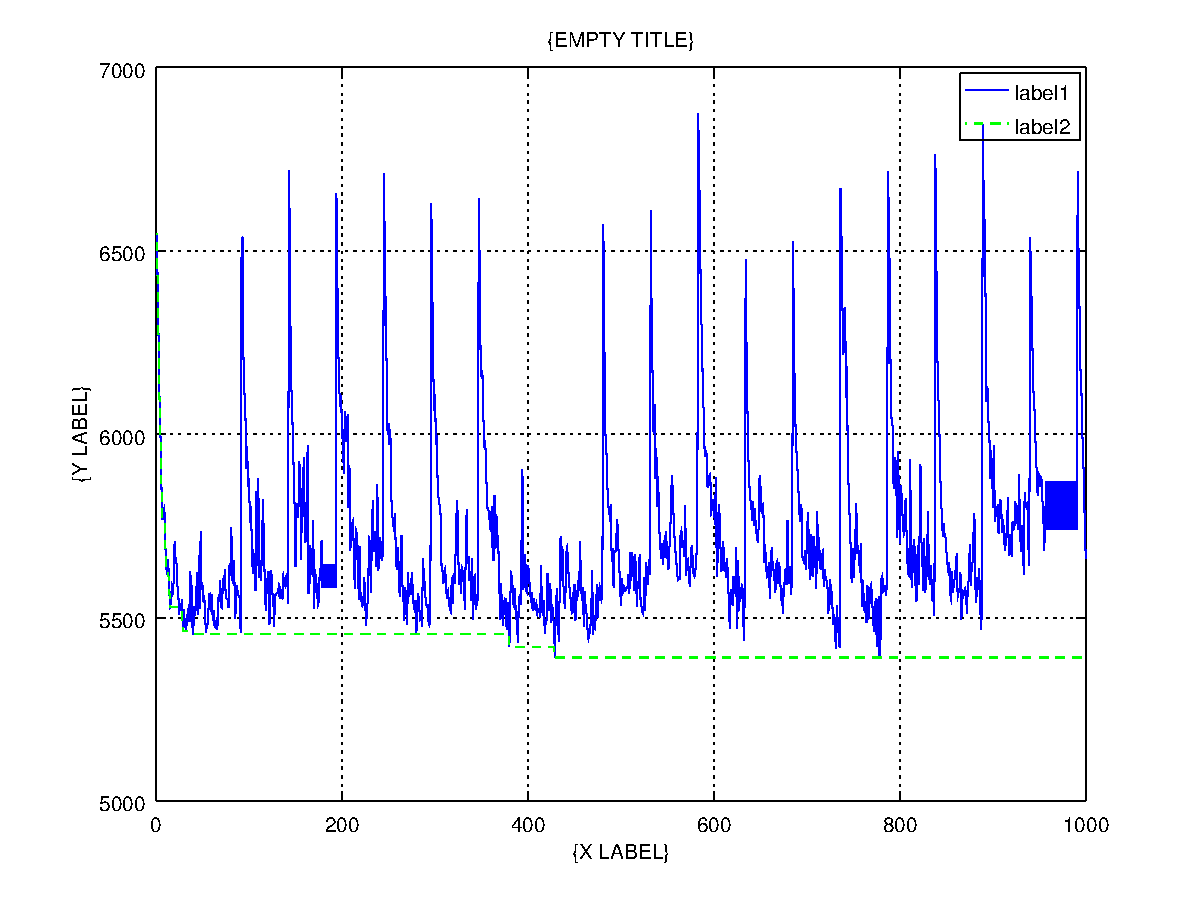
\includegraphics[width=0.67\textwidth]{Appendix_I/GENERATE-PLOT-example/1}
	\hfill\null
	\caption{
		Wygenerowany wykres dwóch funkcji dla przykładowego wywołania skryptu \textsc{generatePlot.bash}, obrazujący sposób zachowania się algorytmu \textsc{Tabu Search} dla przykładowej instancji grafu $G = \left( V, E \right)$, gdzie $\left| V \right| = 30$ ($G$ jest grafem pełnym), dla okresu szukania rozwiązania równego $50$ (po którym następuje ,,restart'' algorytmu).
	}
	\label{fig:genplot}
\end{figure}

\section{Możliwości biblioteki}

Tak jak wspomnieliśmy na samym początku tego rozdziału, biblioteka \textsc{RIT} implementuje wiele z, dotąd przez nas poznanych, algorytmów. Aby zaprezentować możliwość ich wykorzystania, przedstawimy kilka przypadków działania aplikacji, gdzie każdym z~nich będziemy starali odpowiedzieć się na jedno z~podstawowych pytań, jakie mogą się nasunąć podczas zapoznawania się ze strukturą wspomnianej biblioteki. Należy mieć na uwadze, że prezentowane w~tej części wycinki kodu źródłowego, w~charakterze odpowiedzi na każde z~zadanych przez nas pytań, nie są odpowiedziami jedynymi słusznymi --- większość obiektów, jakie będziemy prezentować, biblioteka \textsc{RIT} pozwala stworzyć na więcej niż jeden sposób. My zaś będziemy starali się prezentować tylko te przypadki użycia, które naszym zdaniem pojawiać się mogą najczęściej przy korzystaniu z~niej.

\subsection{Budowanie grafu}

Podstawową czynnością jaką musimy mieć możliwość wykonać, jest budowa grafu, na którym będziemy mogli operować. 

\subsubsection{W jaki sposób zbudować graf przy wykorzystaniu udostępnionych funkcji?}

Biblioteka \textsc{RIT} zapewnia kilka sposobów na generowanie grafów, dla których będziemy później chcieli wykonywać obliczenia. Główne z~nich to:
\begin{itemize}
	\item odczytanie definicji całego grafu z~pliku --- główne z~obsługiwanych formatów opiszemy poniżej, na tę chwilę jesteśmy zainteresowani tylko sposobem wywołania danej funkcjonalności\footnote{W prezentowanych przypadkach użycia pomijamy obsługę wyjątków, zgłaszanych w~czasie wykonywania programu, przykładowo prezentując sposób ich przechwytywania tylko w~pierwszym z~nich.}:
	
	\begin{minted}[escapeinside=||,mathescape=true,linenos=true,fontsize=\footnotesize]{c++}
#include <RIT/exp/IOExceptions.hpp>
#include <RIT/utils/enums/InputFormat.hpp>
#include <RIT/utils/enums/InputMode.hpp>
#include <RIT/utils/IOUtils.hpp>
#include <RIT/utils/MemoryUtils.hpp>

int main() {
	GraphIF* g { };
	try {
		g = InputUtils::readGraph("ścieżka do pliku *.gr", InputFormat::GR, InputMode::HDD);
		MemoryUtils::removeGraph(g, true, true);
	} catch (IOExceptions::FileNotFountException& e) {
		return 0;
	}
	return 0;
}
	\end{minted}
	
	gdzie wartość enumerowana \mintinline{C++}|InputFormat| odpowiada za format, który zdecydowaliśmy się wczytać do programu, \mintinline{C++}|InputMode| --- za sposób jego załadowania, gdzie \mintinline{C++}|HDD| odpowiada standardowej metodzie odczytu pliku, której będziemy używać. Należy oczywiście pamiętać o~usunięciu przed chwilą stworzonego grafu najwcześniej jak to tylko możliwe, jeżeli chcemy ustrzec się przed późniejszymi problemami związanymi z~zarządzaniem pamięcią przez program (każdy prezentowany przykład będzie zawierać również kod usuwający stworzone przez siebie obiekty).
	\item dynamiczna konstrukcja grafu --- umożliwia stworzenie dowolnej struktury grafowej przy wykorzystaniu metod, udostępnianych przez bibliotekę. Poniżej widoczny przykład przedstawia sposób stworzenia grafu z~trzema wierzchołkami, gdzie każdy z~nich jest połączony z~pozostałymi (graf pełny). Dla danej klasy \mintinline{C++}|GraphIF|, podobnie jak dla zdecydowanej większości obiektów, które będziemy wykorzystywać w~prezentowanych kodach, jest dostępna większa liczba konstruktorów --- sposób generowania grafu dla każdego z~nich różni się od poniższego. W~tym konkretnym przypadku graf jest budowany na podstawie dwóch zbiorów danych: jego wierzchołków $V$ oraz, łączących je, krawędzi $E$. Poniżej prezentowany sposób konstrukcji grafu $G = \left( V, E \right)$ jest zatem naturalny:
	
	\begin{minted}[escapeinside=||,mathescape=true,linenos=true,fontsize=\footnotesize]{c++}
VertexSetIF* vSet = new VertexSetImpl { 3 };
EdgeSetIF* eSet = new EdgeSetImpl { 3 };
GraphIF* g = new GraphImpl { vSet, eSet };

for (unsigned int idx = 0; idx < 3; idx += 1) {
	vSet->push_back(new VertexImpl { idx });
}

for (unsigned int idx = 0; idx < 3; idx += 1) {
	eSet->push_back(
		new EdgeImpl { idx, VertexPair(vSet->getElementAt(idx),
			vSet->getElementAt((idx + 1) % 3)), (EdgeCost) idx });
}
MemoryUtils::removeGraph(g, true, true);
	\end{minted}
	gdzie kolejno stworzyliśmy trzy wierzchołki grafu, później zaś, z~wykorzystaniem operacji wyznaczania reszty z~dzielenia,  jego krawędzie: $e_{01}$, $e_{12}$ oraz $e_{20}$, gdzie koszt każdej z~nich wynosi \mintinline{C++}|idx|.\\
	
	\item losowe generowanie struktury --- udostępnione przez klasę pomocniczą \mintinline{C++}|GraphUtils| funkcje, umożliwiają między innymi wygenerowanie losowego grafu na podstawie takich danych jak:
	\begin{itemize}
		\item liczba wierzchołków docelowego grafu,
		\item liczba krawędzi / gęstość grafu (jedna z~dwóch informacji),
		\item najniższy możliwy koszt łuku,
		\item największa waga, jaką może przyjąć krawędź.
	\end{itemize}

	\begin{minted}[escapeinside=||,mathescape=true,linenos=true,fontsize=\footnotesize]{c++}
GraphIF* g = GraphUtils::getRandomGraph(10,0.5,10,15);

MemoryUtils::removeGraph(g, true, true);
	\end{minted}
	gdzie pierwszymi dwoma parametrami w~tym przypadku są: liczba krawędzi oraz gęstość grafu. Powyższy fragment kodu został wykorzystany do wygenerowania wszystkich instancji grafów, dla których zostały przeprowadzone eksperymenty w~rozdziale \ref{ch:exp} (oczywiście dla różnych wartości argumentów).	
\end{itemize}

\subsubsection{Jakie formaty wejściowe obsługuje biblioteka?}

Biblioteka \textsc{RIT} posługuje się istniejącym standardem zapisu informacji grafowych, jaki zastosowano podczas dziewiątej edycji programu \textsc{DIMACS Implementation Challenge}, która skupiała się na problemie wyszukiwania najkrótszych ścieżek w~grafach. Wykorzystanie tej struktury dla problemu minimalnego drzewa rozpinającego nie stanowi żadnej trudności, gdyż oba te problemy są oczywiście problemami grafowymi. Przykładowy plik, zawierający opis grafu, jego wierzchołków oraz krawędzi, wygląda tak, jak pokazano poniżej:

\begin{minted}[escapeinside=||,mathescape=true,linenos=true,fontsize=\footnotesize]{text}
c 9th DIMACS Implementation Challenge: Shortest Paths
c http://www.dis.uniroma1.it/|\textapprox|challenge9
c Sample graph file
c
p |\textbf{mst}| 6 8
c graph contains 6 nodes and 8 arcs
c node ids are numbers in 0..5
c
a 0 1 17
c arc from node 0 to node 1 of weight 17
c
a 0 2 10
a 1 3 2
a 2 4 0
a 3 2 0
a 3 5 3
a 4 1 0
a 4 5 20
\end{minted}
gdzie pierwsza litera rozpoczynająca nową linię, niesie za sobą informację co w~dane linii można znaleźć. Opisując każdą z~nich po kolei mamy:

\begin{itemize}
	\item[c] --- linie zawierające dowolny komentarz, nie dłuższy jednak niż \mintinline{C++}|IOUtils::impl::MAX_CHARS_IN_LINE| (stała biblioteki \textsc{RIT\_Library}, definiowana ze względów optymalizacji procesu samego odczytywania pliku),
	\item[p] --- linia, rozpoczynająca się takim symbolem, zawiera definicję problemu, który dany plik opisuje. W~naszym przypadku jest to problem minimalnego drzewa rozpinającego (\textbf{mst}),
	\item[a] --- trzy liczby, które znajdują się w~każdej linii, rozpoczynającej się od tego znaku, znaczą kolejno:
	\begin{itemize}
		\item numer wierzchołka, z~którego definiowana krawędź wychodzi (gdzie wierzchołki numerowane są od zera),
		\item identyfikator drugiego węzła z~pary dla krawędzi (krawędzie są nieskierowane, więc kolejność zapisu wierzchołków jest umowna),
		\item koszt definiowanej krawędzi.
	\end{itemize}
\end{itemize}

\subsubsection{Jak zapisać wygenerowany graf?}

W celu zapisania do pliku grafu, wygenerowanego jedną z~dwóch ostatnich opisanych przez nas metod, należy posłużyć się poniżej prezentowanym fragmentem kodu:

\begin{minted}[escapeinside=||,mathescape=true,linenos=true,fontsize=\footnotesize]{c++}
GraphIF* g = GraphUtils::getRandomGraph(10,0.5,10,15);

OutputUtils::exportGraph(g, "ścieżka do pliku", OutputFormat::GR);

MemoryUtils::removeGraph(g, true, true);
\end{minted}

\subsection{Rozwiązywanie problemów grafowych}

Wszystkie prezentowane przypadki użycia, pozwalające na rozwiązywanie problemów grafowych, mają bardzo podobną do siebie budowę. Uruchomienie procesu poszukiwania minimalnego drzewa rozpinającego dla grafu $G$ wymaga od nas stworzenia instancji obiektu, który implementuje odpowiednie dla każdego problemu metody. Wszystkie obiekty, którymi będziemy się posługiwać, mają budowę, pozwalającą na bardzo łatwą manipulację nimi. Przykładem takiego obiektu jest \mintinline{C++}|MSTSolverImpl| (razem z~podobnymi sobie dalej nazywany krótko \textit{solverem}),

\begin{minted}[escapeinside=||,mathescape=true,linenos=true,fontsize=\footnotesize]{c++}
GraphIF* g = GraphUtils::getRandomGraph(10, 0.5, 10, 15);
MSTSolverIF* mstSolver = new MSTSolverImpl { g };

delete mstSolver;
MemoryUtils::removeGraph(g, true, true);
\end{minted}
który swoją definicję opiera na zawartości pliku nagłówkowego \mintinline{C++}|<RIT/mstsolver/MSTSolverInclude.hpp>|, który wygląda następująco: 

\begin{minted}[escapeinside=||,mathescape=true,linenos=true,fontsize=\footnotesize]{c++}
#ifndef SRC_INCLUDE_MSTSOLVER_MSTSOLVERINCLUDE_HPP_
#define SRC_INCLUDE_MSTSOLVER_MSTSOLVERINCLUDE_HPP_

#define MSTSolverIF_PrimeHeap

#include "MSTSolverIF.hpp"

#ifdef MSTSolverIF_PrimeHeap
#include "PrimeHeap.hpp"
#elif defined(MSTSolverIF_Kruskal)
#include "Kruskal.hpp"
#endif

typedef PrimeHeap MSTSolverImpl;

#endif /* SRC_INCLUDE_MSTSOLVER_MSTSOLVERINCLUDE_HPP_ */
\end{minted}

Ten oraz znaczna część obiektów, które implementuje biblioteka \textsc{RIT}, jest przedstawiona właśnie w~taki sposób. Taka modularna budowa biblioteki \textsc{RIT} umożliwia szybką zmianę implementacji praktycznie dowolnej struktury, która jest wykorzystywana w~aplikacji, bez potrzeby jej przebudowywania (w takiej sytuacji od użytkownika wymaga się jedynie podmiany dwóch linii odpowiedniego pliku nagłówkowego by przedefiniować dany typ obiektu na inny).

Inną możliwością wyboru odpowiedniego narzędzia jest skorzystanie z~klasy pomocniczej \mintinline{C++}|SolverFactory|, która bazuje na identycznym rozwiązaniu, co przedstawione powyżej, jednak pozwala na dużo wygodniejszą formę pracy z~aplikacją.

\subsubsection{Jak rozwiązać problem minimalnego drzewa rozpinającego?}

Aby rozwiązać dowolną instancję zadanego problemu, możemy posłużyć się poniższym przykładem, który generuje przykładowy graf, tworzy domyślną (\mintinline{C++}|MSTSolverEnum::DEFAULT|) klasę \textit{solvera}, dostarcza nam rozwiązanie problemu, wypisuje je a~na końcu usuwa wszystkie obiekty z~pamięci:

\begin{minted}[escapeinside=||,mathescape=true,linenos=true,fontsize=\footnotesize]{c++}
GraphIF* g = GraphUtils::getRandomGraph(10, 0.5, 10, 15);
MSTSolverIF* mstSolver = SolverFactory::getMSTSolver(MSTSolverEnum::DEFAULT, g);
EdgeSetIF* solution = mstSolver->getMST();

std::cout << solution->toString() << std::endl;
std::cout << solution->getTotalEdgeCost() << std::endl;

MemoryUtils::removeCollection(solution, false);
delete mstSolver;
MemoryUtils::removeGraph(g, true, true);
\end{minted}

Oprócz takich klasycznych implementacji jak algorytm Prima czy Kruskala, biblioteka \textsc{RIT} umożliwia nam rozwiązanie tych samych problemów za pomocą programowania liniowego bądź całkowitoliczbowego. Do poprawnego funkcjonowania tej części funkcjonalności niezbędny jednak jest pakiet optymalizacyjny \textsc{IBM\textsuperscript{\textregistered} CPLEX\textsuperscript{\textregistered} Optimizer}. Z~uwagi na powyższy fakt, klasy, które umożliwiają dostęp do tego typu \textit{solverów}, nie mają wspólnego interfejsu z~pozostałymi obiektami, tak aby można było łatwo usunąć z~projektu biblioteki \textsc{RIT} kłopotliwe zależności (np. w~przypadku braku owego pakietu).

\begin{minted}[escapeinside=||,mathescape=true,linenos=true,fontsize=\footnotesize]{c++}
GraphIF* g = GraphUtils::getRandomGraph(10, 0.5, 10, 15);
CPLEX_LP_MSTSolverIF* lpMstSolver = new CPLEX_LP_MSTSolverImpl { g };
//MSTSolverIF* mstSolver = SolverFactory::getMSTSolver(MSTSolverEnum::DEFAULT, g);
//EdgeSetIF* solution = mstSolver->getMST();
EdgeSetIF* solution = lpMstSolver->getMST();

std::cout << solution->toString() << std::endl;
std::cout << solution->getTotalEdgeCost() << std::endl;

MemoryUtils::removeCollection(solution, false);
delete lpMstSolver;
//delete mstSolver;
MemoryUtils::removeGraph(g, true, true);
\end{minted}

W powyższym kodzie celowo pozostawiono komentarze, aby uwypuklić fakt prostoty zamiany jednego algorytmu na inny. Choć powiedzieliśmy, że obiekty, które opierają się na pakiecie \textsc{IBM\textsuperscript{\textregistered} CPLEX\textsuperscript{\textregistered} Optimizer}, nie mają części wspólnej z~pozostałymi klasami, implementują one niemal te same interfejsy, dzięki którym możemy zminimalizować liczbą potrzebnych do wykonania zmian, w~przypadku chęci wykorzystania innego typu \textit{solvera}.

\subsubsection{Jak rozwiązać problem minimalnego drzewa rozpinającego w~wersji INCREMENTAL?}

Poniżej przedstawiono przykładowy kod, dzięki któremu szybko można zacząć pracę z~problemami typu \textsc{Incremental Minimum Spanning Tree}. Jak możemy się przekonać, nic nie stoi na przeszkodzie by łączyć wiele różnych instancji \textit{solverów} w~jednym ciągu obliczeń, mając dodatkowo wpływ na rodzaj każdego z~nich (poprzez edycję plików \mintinline{C++}|<RIT/mstsolver/MSTSolverInclude.hpp>| oraz \mintinline{C++}|<RIT/imstsolver/IMSTSolverInclude.hpp>| lub posługiwanie się klasą \mintinline{C++}|SolverFactory|):

\begin{minted}[escapeinside=||,mathescape=true,linenos=true,fontsize=\footnotesize]{c++}
IncrementalParam k = 5;
GraphIF* g = GraphUtils::getRandomGraph(10, 0.5, 10, 15);
MSTSolverIF* mstSolver = SolverFactory::getMSTSolver(MSTSolverEnum::DEFAULT, g);
IMSTSolverIF* imstSolver = SolverFactory::getIMSTSolver(IMSTSolverEnum::DEFAULT, g);
EdgeSetIF* baseSolution = mstSolver->getMST();
delete mstSolver;

EdgeSetIF* solution = imstSolver->getIMST(k, baseSolution);
MemoryUtils::removeCollection(baseSolution, false);

std::cout << solution->toString() << std::endl;
std::cout << solution->getTotalEdgeCost() << std::endl;

MemoryUtils::removeCollection(solution, false);
delete imstSolver;
MemoryUtils::removeGraph(g, true, true);
\end{minted}

Analogicznie do problemu minimalnego drzewa rozpinającego możemy dla powyższego kodu skonstruować jego odpowiednik, który w~całości będzie oparty o~pakiet optymalizacyjny \textsc{IBM\textsuperscript{\textregistered} CPLEX\textsuperscript{\textregistered} Optimizer}. Należy mieć jednak świadomość tego, że takie rozwiązanie będzie dużo mniej wydajne niż prezentowane i~zostało zaimplementowane jedynie w~celu potwierdzenia poprawności działania pozostałych \textit{solverów}.

\subsubsection{Jak rozwiązać problem adwersarza?}

W celu rozwiązania problemu adwersarza potrzebujemy dodatkowo wczytać do programu sam zestaw scenariuszy, z~których to algorytm będzie korzystał. Przykład, jak to zrobić, jest prezentowany poniżej:

\begin{minted}[escapeinside=||,mathescape=true,linenos=true,fontsize=\footnotesize]{c++}
IncrementalParam k = 5;
GraphIF* g = InputUtils::readGraph("ścieżka do pliku *.gr", InputFormat::GR, InputMode::HDD);
GraphEdgeCostsSet adversarialScenarios { };
MSTSolverIF* mstSolver = SolverFactory::getMSTSolver(g);
AIMSTSolution aimstSolution { };
AIMSTSolverIF* aimstSolver = SolverFactory::getAIMSTSolver(g,
adversarialScenarios, k);

EdgeSetIF* baseSolution = mstSolver->getMST();
delete mstSolver;

EdgeSetIF* solution { };

for (int i = 1; i < 10; i += 1) {
	adversarialScenarios.insert(
		InputUtils::readCosts("ścieżka do pliku *.gr", InputFormat::GR, InputMode::HDD)
	);
}

aimstSolution = aimstSolver->getMST(baseSolution);
solution = AIMSTUtils::getEdgeSet(aimstSolution);

MemoryUtils::removeCollection(baseSolution, false);
delete aimstSolver;

std::cout << solution->toString() << std::endl;
std::cout << solution->getTotalEdgeCost() << std::endl;

MemoryUtils::removeCollection(solution, false);
MemoryUtils::removeScenarioSet(adversarialScenarios);
MemoryUtils::removeGraph(g, true, true);
\end{minted}

\subsubsection{Jak rozwiązać problem odpornej optymalizacji z~możliwością poprawy?}

Tak jak w~przypadku odpowiedzi na wszystkie poprzednie pytania, tak i~tutaj zaprezentujemy przykładowy kod, dzięki któremu możliwe jest szybkie wczytanie danych dla problemu \textsc{Recoverable Robust Incremental Spanning Tree} oraz uruchomienie algorytmu \textsc{Tabu Search}, który jest domyślną implementacją obiektu, rozwiązującego dane zagadnienie (zwracającego rozwiązanie jak najbliższe optymalnego).
\begin{minted}[escapeinside=||,mathescape=true,linenos=true,fontsize=\footnotesize]{c++}
IncrementalParam k { 5 };
TabuIterationCount tabuPeriod { 100 };
TabuIterationCount numberOfPathIterations { 50 };
TabuIterationCount numberOfIterations { 2000 };

GraphIF* g = InputUtils::readGraph("ścieżka do pliku *.gr", InputFormat::GR,
InputMode::HDD);
GraphEdgeCostsSet adversarialScenarios { };
RIMSTSolverIF* rimstSolver = new RIMSTSolverImpl { AIMSTSolverEnum::DEFAULT,
	IMSTSolverEnum::DEFAULT, MSTSolverEnum::DEFAULT, g, adversarialScenarios, k, 
	tabuPeriod, numberOfPathIterations, numberOfIterations
};

for (int i = 1; i < 10; i += 1) {
	adversarialScenarios.insert(
		InputUtils::readCosts("ścieżka do pliku *.gr", InputFormat::GR, InputMode::HDD)
	);
}

EdgeSetIF* solution = rimstSolver->getMST();
delete rimstSolver;

std::cout << solution->toString() << std::endl;
std::cout << solution->getTotalEdgeCost() << std::endl;

MemoryUtils::removeCollection(solution, false);
MemoryUtils::removeScenarioSet(adversarialScenarios);
MemoryUtils::removeGraph(g, true, true);
\end{minted}

\section{Przykładowa sesja}\label{sec:logging}

Poniżej zaprezentowano zapis zdarzeń, powstały w~wyniku uruchomienia algorytmu dla problemu \textsc{Incremental Minimum Spanning Tree}, dla grafu o~$5$ wierzchołkach i~$6$ krawędziach, gdzie zapisywanymi informacjami są tylko te zdarzenia, których źródło znajduje się w~jednym z~plików: \textsc{IMSTSolverIF.cpp} lub \textsc{BinarySearch\_v2.cpp} (wszystkie inne zostały pominięte).

\begin{minted}[escapeinside=||,mathescape=true,linenos=true,fontsize=\tiny]{text}
[...]
2016-06-19 18:45:29,123 INFO  IMSTSolverIF (../src/src/imstsolver/IMSTSolverIF.cpp:59) - No new base edge set was used. Running Incremental MST Solver on previous solution:
	(0)	<------- [	3	] ------->	(1)
	(1)	<------- [	3	] ------->	(2)
	(2)	<------- [	5	] ------->	(3)
	(4)	<------- [	2	] ------->	(3)
with total edge costs: 13.000000000.
2016-06-19 18:45:29,124 INFO  IMSTSolverIF (../src/src/imstsolver/IMSTSolverIF.cpp:68) - New set of edges' costs has been given. Changing costs of edges as shown below:
	(0)	<------- [	3	==>	4	] ------->	(1)
	(3)	<------- [	8	==>	6	] ------->	(0)
	(1)	<------- [	6	==>	1	] ------->	(4)
	(4)	<------- [	2	==>	9	] ------->	(3)
	(2)	<------- [	5	==>	7	] ------->	(3).
2016-06-19 18:45:29,125 INFO  BinarySearch_v2 (../src/src/imstsolver/BinarySearch_v2.cpp:345) - There are some changes it costs of graph's edges. 
	New unbounded solution will be calculated for k parameter value: 1.
2016-06-19 18:45:29,126 INFO  IMSTSolverIF (../src/src/imstsolver/IMSTSolverIF.cpp:101) - New MST solution has given set of edges that is not a part of original solution:
	(1)	<------- [	1	] ------->	(4)
	(3)	<------- [	6	] ------->	(0).
Total number of edges in set: 2.
2016-06-19 18:45:29,126 INFO  BinarySearch_v2 (../src/src/imstsolver/BinarySearch_v2.cpp:360) - Unbounded solution that was found has got unacceptable number of edges 
	that are not in base solution. Looking for 1-bounded optimal solution for Incremental MST problem...
2016-06-19 18:45:29,126 INFO  BinarySearch_v2 (../src/src/imstsolver/BinarySearch_v2.cpp:51) - Generating graph that contains smaller set of edges 
	based on base edge set (with 4 edges):
	(0)	<------- [	4	] ------->	(1)
	(1)	<------- [	3	] ------->	(2)
	(2)	<------- [	7	] ------->	(3)
	(4)	<------- [	9	] ------->	(3),
and k-unbounded edge set that forms MST solution (4 edges):
	(0)	<------- [	4	] ------->	(1)
	(1)	<------- [	1	] ------->	(4)
	(1)	<------- [	3	] ------->	(2)
	(3)	<------- [	6	] ------->	(0).
2016-06-19 18:45:29,128 INFO  BinarySearch_v2 (../src/src/imstsolver/BinarySearch_v2.cpp:84) - Graph with 5 vertices and the following set of edges 
	was generated (with 6 edges) and will be used to solve MST in Incremental version:
	(0)	<------- [	4	] ------->	(1)
	(3)	<------- [	6	] ------->	(0)
	(1)	<------- [	1	] ------->	(4)
	(4)	<------- [	9	] ------->	(3)
	(1)	<------- [	3	] ------->	(2)
	(2)	<------- [	7	] ------->	(3).
2016-06-19 18:45:29,130 INFO  BinarySearch_v2 (../src/src/imstsolver/BinarySearch_v2.cpp:93) - Edge preprocessing. Cost of every edge 
	in shrunken graph (6 edges) will be temporary changed as follows:
		c'_{e_{i}} = c_{e_{i}} + (mi^2 + i)/(m + 1)^3.
2016-06-19 18:45:29,130 INFO  BinarySearch_v2 (../src/src/imstsolver/BinarySearch_v2.cpp:101) - Temporary changing edge cost as follows:
	(0)	<------- [	4	==>	4.02041	] ------->	(1).
2016-06-19 18:45:29,130 INFO  BinarySearch_v2 (../src/src/imstsolver/BinarySearch_v2.cpp:101) - Temporary changing edge cost as follows:
	(3)	<------- [	6	==>	6.0758	 ] ------->	(0).
2016-06-19 18:45:29,131 INFO  BinarySearch_v2 (../src/src/imstsolver/BinarySearch_v2.cpp:101) - Temporary changing edge cost as follows:
	(1)	<------- [	1	==>	1.16618	] ------->	(4).
2016-06-19 18:45:29,131 INFO  BinarySearch_v2 (../src/src/imstsolver/BinarySearch_v2.cpp:101) - Temporary changing edge cost as follows:
	(4)	<------- [	9	==>	9.29155	] ------->	(3).
2016-06-19 18:45:29,131 INFO  BinarySearch_v2 (../src/src/imstsolver/BinarySearch_v2.cpp:101) - Temporary changing edge cost as follows:
	(1)	<------- [	3	==>	3.4519	 ] ------->	(2).
2016-06-19 18:45:29,132 INFO  BinarySearch_v2 (../src/src/imstsolver/BinarySearch_v2.cpp:101) - Temporary changing edge cost as follows:
	(2)	<------- [	7	==>	7.64723	] ------->	(3).
2016-06-19 18:45:29,132 TRACE BinarySearch_v2 (../src/src/imstsolver/BinarySearch_v2.cpp:125) - Generating data to calculate |$\lambda$| parameters.
2016-06-19 18:45:29,132 INFO  BinarySearch_v2 (../src/src/imstsolver/BinarySearch_v2.cpp:141) - Based on original MST solution's edges:
	(0)	<------- [	4.02041	] ------->	(1)
	(1)	<------- [	3.4519	 ] ------->	(2)
	(2)	<------- [	7.64723	] ------->	(3)
	(4)	<------- [	9.29155	] ------->	(3)
with 4 edges, MST for new costs:
	(0)	<------- [	4.02041	] ------->	(1)
	(1)	<------- [	1.16618	] ------->	(4)
	(1)	<------- [	3.4519	 ] ------->	(2)
	(3)	<------- [	6.0758 	] ------->	(0)
with 4 edges, following sets was generated:
T^{0} \ T^{*} (edges that are only in old solution - 2 edges):
	(4)	<------- [	9.29155	] ------->	(3)
	(2)	<------- [	7.64723	] ------->	(3),
T^{*} \ T^{0} (edges that are only in new solution - 2 edges):
	(3)	<------- [	6.0758	 ] ------->	(0)
	(1)	<------- [	1.16618	] ------->	(4).
2016-06-19 18:45:29,135 TRACE BinarySearch_v2 (../src/src/imstsolver/BinarySearch_v2.cpp:145) - Generating set of edges 
	that are in complementary set of original and new minimum spanning tree sets.
2016-06-19 18:45:29,136 TRACE BinarySearch_v2 (../src/src/imstsolver/BinarySearch_v2.cpp:154) - Sorting generated set in ascending order.
2016-06-19 18:45:29,136 TRACE BinarySearch_v2 (../src/src/imstsolver/BinarySearch_v2.cpp:165) - Generating set of edges 
	that are in complementary set of new and original minimum spanning tree sets.
2016-06-19 18:45:29,136 TRACE BinarySearch_v2 (../src/src/imstsolver/BinarySearch_v2.cpp:174) - Sorting generated set in descending order.
2016-06-19 18:45:29,136 INFO  BinarySearch_v2 (../src/src/imstsolver/BinarySearch_v2.cpp:187) - Checking correctness lower and upper bounds of |$\lambda$| parameter...
2016-06-19 18:45:29,136 INFO  BinarySearch_v2 (../src/src/imstsolver/BinarySearch_v2.cpp:210) - Using default |$\lambda$| bounds:
	[1.571428571	:	8.125364431].
2016-06-19 18:45:29,136 INFO  BinarySearch_v2 (../src/src/imstsolver/BinarySearch_v2.cpp:421) - Performing Incremental MST binary search. 
	Generating indexes of |$\lambda$| parameter feasible set...
2016-06-19 18:45:29,136 INFO  BinarySearch_v2 (../src/src/imstsolver/BinarySearch_v2.cpp:426) - Incremental MST binary search 
	will start new iteration with initial |$\lambda$| bounds:
	[1.571428571:	8.125364431	].
2016-06-19 18:45:29,136 TRACE BinarySearch_v2 (../src/src/imstsolver/BinarySearch_v2.cpp:433) - Generating lower indexes for feasible |$\lambda$| parameter set, 
	starting with |$\lambda$|(1, 0) (while first parameter will be decreasing, second - increasing).
2016-06-19 18:45:29,137 TRACE BinarySearch_v2 (../src/src/imstsolver/BinarySearch_v2.cpp:437) - Performing search for minimal index 'j' such that:
	|$\lambda$|_{LB}	<=	|$\lambda$|(1,j),
	|$\lambda$|_{LB}	=	1.571428571.
2016-06-19 18:45:29,137 TRACE BinarySearch_v2 (../src/src/imstsolver/BinarySearch_v2.cpp:448) - Minimal index 'j' such that:
	|$\lambda$|_{LB}	<=	|$\lambda$|(1,j),
	|$\lambda$|_{LB}	=	1.571428571
has been found and it equals 0 (3.215743440).
2016-06-19 18:45:29,137 TRACE BinarySearch_v2 (../src/src/imstsolver/BinarySearch_v2.cpp:437) - Performing search for minimal index 'j' such that:
	|$\lambda$|_{LB}	<=	|$\lambda$|(0,j),
	|$\lambda$|_{LB}	=	1.571428571.
2016-06-19 18:45:29,138 TRACE BinarySearch_v2 (../src/src/imstsolver/BinarySearch_v2.cpp:448) - Minimal index 'j' such that:
	|$\lambda$|_{LB}	<=	|$\lambda$|(0,j),
	|$\lambda$|_{LB}	=	1.571428571
has been found and it equals 0 (1.571428571).
2016-06-19 18:45:29,138 TRACE BinarySearch_v2 (../src/src/imstsolver/BinarySearch_v2.cpp:462) - Generating upper indexes for feasible |$\lambda$| parameter set,
	starting with |$\lambda$|(0, 1) (while first parameter will be increasing, second - decreasing).
2016-06-19 18:45:29,138 TRACE BinarySearch_v2 (../src/src/imstsolver/BinarySearch_v2.cpp:466) - Performing search for maximal index 'j' such that:
	|$\lambda$|(0,j)	<=	|$\lambda$|_{UB},
	|$\lambda$|_{UB}	=	8.125364431.
2016-06-19 18:45:29,139 TRACE BinarySearch_v2 (../src/src/imstsolver/BinarySearch_v2.cpp:474) - Maximal index 'j' such that:
	|$\lambda$|(0,j)	<=	|$\lambda$|_{UB},
	|$\lambda$|_{UB}	=	8.125364431
has been found and it equals 1 (6.481049563).
2016-06-19 18:45:29,139 TRACE BinarySearch_v2 (../src/src/imstsolver/BinarySearch_v2.cpp:466) - Performing search for maximal index 'j' such that:
	|$\lambda$|(1,j)	<=	|$\lambda$|_{UB},
	|$\lambda$|_{UB}	=	8.125364431.
2016-06-19 18:45:29,139 TRACE BinarySearch_v2 (../src/src/imstsolver/BinarySearch_v2.cpp:474) - Maximal index 'j' such that:
	|$\lambda$|(1,j)	<=	|$\lambda$|_{UB},
	|$\lambda$|_{UB}	=	8.125364431
has been found and it equals 1 (8.125364431).
2016-06-19 18:45:29,140 TRACE BinarySearch_v2 (../src/src/imstsolver/BinarySearch_v2.cpp:487) - Counting feasible |$\lambda$| parameters...
2016-06-19 18:45:29,140 TRACE BinarySearch_v2 (../src/src/imstsolver/BinarySearch_v2.cpp:510) - For parameter 'i' (0), 2 expressions of type |$\lambda$|(i,j) 
	was found (from j = 0 to 1) and will be added to feasible solution which size is now 2.
2016-06-19 18:45:29,140 TRACE BinarySearch_v2 (../src/src/imstsolver/BinarySearch_v2.cpp:510) - For parameter 'i' (1), 2 expressions of type |$\lambda$|(i,j) 
	was found (from j = 0 to 1) and will be added to feasible solution which size is now 4.
2016-06-19 18:45:29,140 INFO  BinarySearch_v2 (../src/src/imstsolver/BinarySearch_v2.cpp:525) - Size of generated |$\lambda$| parameter feasible set 
	is small enough (4) to execute |$\lambda$|-based MST binary search (threshold was 4).
2016-06-19 18:45:29,140 TRACE BinarySearch_v2 (../src/src/imstsolver/BinarySearch_v2.cpp:534) - Adding feasible |$\lambda$| parameter which satisfy:
	1.571428571	<=	|$\lambda$|(0, 0)	=	1.571428571	<=	8.125364431.
2016-06-19 18:45:29,141 TRACE BinarySearch_v2 (../src/src/imstsolver/BinarySearch_v2.cpp:534) - Adding feasible |$\lambda$| parameter which satisfy:
	1.571428571	<=	|$\lambda$|(0, 1)	=	6.481049563	<=	8.125364431.
2016-06-19 18:45:29,141 TRACE BinarySearch_v2 (../src/src/imstsolver/BinarySearch_v2.cpp:534) - Adding feasible |$\lambda$| parameter which satisfy:
	1.571428571	<=	|$\lambda$|(1, 0)	=	3.215743440	<=	8.125364431.
2016-06-19 18:45:29,141 TRACE BinarySearch_v2 (../src/src/imstsolver/BinarySearch_v2.cpp:534) - Adding feasible |$\lambda$| parameter which satisfy:
	1.571428571	<=	|$\lambda$|(1, 1)	=	8.125364431	<=	8.125364431.
2016-06-19 18:45:29,142 INFO  BinarySearch_v2 (../src/src/imstsolver/BinarySearch_v2.cpp:246) - Executing binary search for 4 |$\lambda$| parameters, sorted in ascending order...
2016-06-19 18:45:29,142 INFO  BinarySearch_v2 (../src/src/imstsolver/BinarySearch_v2.cpp:251) - Searching for a solution in |$\lambda$| parameter space bounded by:
	lower index	:	0,
	lower |$\lambda$| value      :	1.571428571
	upper index	:	3,
	upper |$\lambda$| value      :	8.125364431.
2016-06-19 18:45:29,142 INFO  BinarySearch_v2 (../src/src/imstsolver/BinarySearch_v2.cpp:256) - Calculate MST solution for selected |$\lambda$| parameter:
	index	:	1,
	|$\lambda$| value      :	3.215743440.
2016-06-19 18:45:29,143 INFO  BinarySearch_v2 (../src/src/imstsolver/BinarySearch_v2.cpp:217) - Setting new graph's edges cost based on |$\lambda$| parameter value: 3.215743440...
2016-06-19 18:45:29,143 INFO  BinarySearch_v2 (../src/src/imstsolver/BinarySearch_v2.cpp:224) - Temporary changing edge cost as follows:
	(0)	<------- [	4.02041	==>	0.804665	] ------->	(1).
2016-06-19 18:45:29,143 INFO  BinarySearch_v2 (../src/src/imstsolver/BinarySearch_v2.cpp:224) - Temporary changing edge cost as follows:
	(1)	<------- [	3.4519         ==>	0.236152        ] ------->	(2).
2016-06-19 18:45:29,144 INFO  BinarySearch_v2 (../src/src/imstsolver/BinarySearch_v2.cpp:224) - Temporary changing edge cost as follows:
	(2)	<------- [	7.64723	==>	4.43149	 ] ------->	(3).
2016-06-19 18:45:29,144 INFO  BinarySearch_v2 (../src/src/imstsolver/BinarySearch_v2.cpp:224) - Temporary changing edge cost as follows:
	(4)	<------- [	9.29155	==>	6.0758	  ] ------->	(3).
2016-06-19 18:45:29,144 INFO  IMSTSolverIF (../src/src/imstsolver/IMSTSolverIF.cpp:101) - New MST solution has given set of edges that is not a part of original solution:
	(1)	<------- [	1.16618	] ------->	(4).
Total number of edges in set: 1.
2016-06-19 18:45:29,145 INFO  BinarySearch_v2 (../src/src/imstsolver/BinarySearch_v2.cpp:303) - For |$\lambda$| parameter value 3.215743440 an optimal solution 
	has been found (with total cost of edges: 6.638483965). Solution includes following edges:
	(0)	<------- [	0.804665       ] ------->	(1)
	(1)	<------- [	0.236152       ] ------->	(2)
	(1)	<------- [	1.16618	] ------->	(4)
	(2)	<------- [	4.43149	] ------->	(3)
in which there are 1 edges that are not in base edge set:
	(1)	<------- [	1.16618	] ------->	(4).
\end{minted}